% Author: Alfredo Sánchez Alberca (asalber@ceu.es)

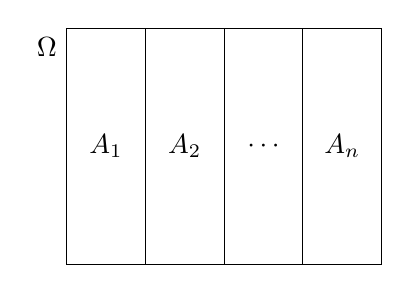
\begin{tikzpicture}
\draw (0,3) node[anchor=north east] {$\Omega$} rectangle (4,0);
\foreach \x in {1,2,3} {
	\draw (\x,0) -- (\x,3);
} 
\node at (0.5,1.5) {$A_1$};
\node at (1.5,1.5) {$A_2$};
\node at (2.5,1.5) {$\cdots$};
\node at (3.5,1.5) {$A_n$};
\end{tikzpicture}